%!TeX program=pdflatex

\documentclass{beamer}
\usetheme{metropolis} 

%PdfTeX settings for a correct UTF 8 Mapping
%------------------------------------------------------
\usepackage{ifpdf}
\ifpdf    \input{glyphtounicode.tex}    %Part of modern distribution
%%%\input{glyphtounicode-cmr.tex}     %Additionnal glyph: You must grab it from pdfx package
\pdfgentounicode=1
\else  %Place here the settings for other compilator
\fi


%Encoding + cmap (to get proper UTF8 mapping)
%------------------------------------------------------
\usepackage{cmap}
\usepackage[utf8]{inputenc}
\usepackage[T1]{fontenc}
\usepackage{lmodern}

%AMS Math + UTF8 mapping of ams symbols
%------------------------------------------------------
\usepackage{amsmath, esint, bm} 
\usepackage{amssymb} % I load it after Fourier else I have more incorrect utf8 mapping (with \geqslant for example)
%Correct UTF8 mapping for ams fonts
\ifdefined\pdffontattr% \ifdefined is part of the e-TeX extension, which is part of any modern LaTeX compiler. 
\immediate\pdfobj stream file {umsa.cmap}
{\usefont{U}{msa}{m}{n}\pdffontattr\font{/ToUnicode \the\pdflastobj\space 0 R}}
\immediate\pdfobj stream file {umsb.cmap}
{\usefont{U}{msb}{m}{n}\pdffontattr\font{/ToUnicode \the\pdflastobj\space 0 R}}
\fi

\usepackage{amsthm, amssymb, bm}
\usepackage{graphicx, caption, subcaption} 
\usepackage{algorithm, algpseudocode}

\graphicspath{{figures/}}

% Environments: definition, example, theorem, lemma, corollary, proposition, remark
\theoremstyle{plain}
\newtheorem{proposition}{Proposition}
\theoremstyle{remark}
\newtheorem{remark}{Remark} 
 
\title{Computational methods for polypeptide origami design}
\author{Daniel Silađi}
\institute{Mentor: Andrej Brodnik\\
Co-mentor: Rok Požar}
\date{}

\begin{document}

\frame{\titlepage}

\section{Introduction}

\begin{frame}{Talk structure}
	\begin{itemize}
		\item Mathematical and biochemical background
		\item Interaction graphs and orthogonal sets
		\item An exact algorithm for the maximum orthogonal set problem
		\item Some heuristics for the maximum orthogonal set problem
		\item Results and conclusions
	\end{itemize}
\end{frame}

\section{Biochemical background}

\begin{frame}{Inspiration -- DNA origami}
	By prescribing the sequence of bases in a single strand of DNA, we can build complex 2D and even 3D nanostructures
	\begin{figure}
		\centering
		\begin{subfigure}{0.45\textwidth}
			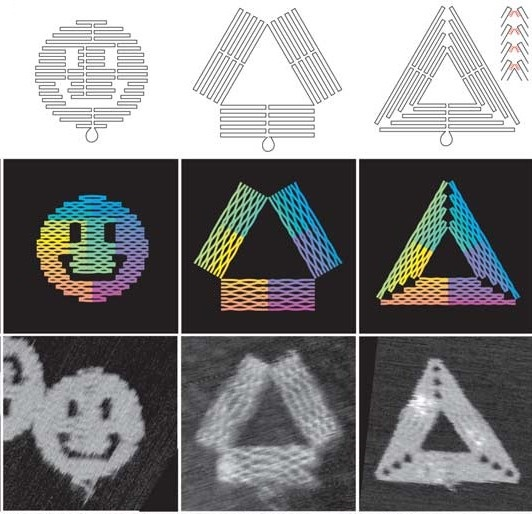
\includegraphics[width=\linewidth]{figures/DNA_origami_cropped_more.png}
			\caption{2D DNA origami, from the original paper, \cite{rothemund2006folding}}
		\end{subfigure}
		~
		\begin{subfigure}{0.45\textwidth}
			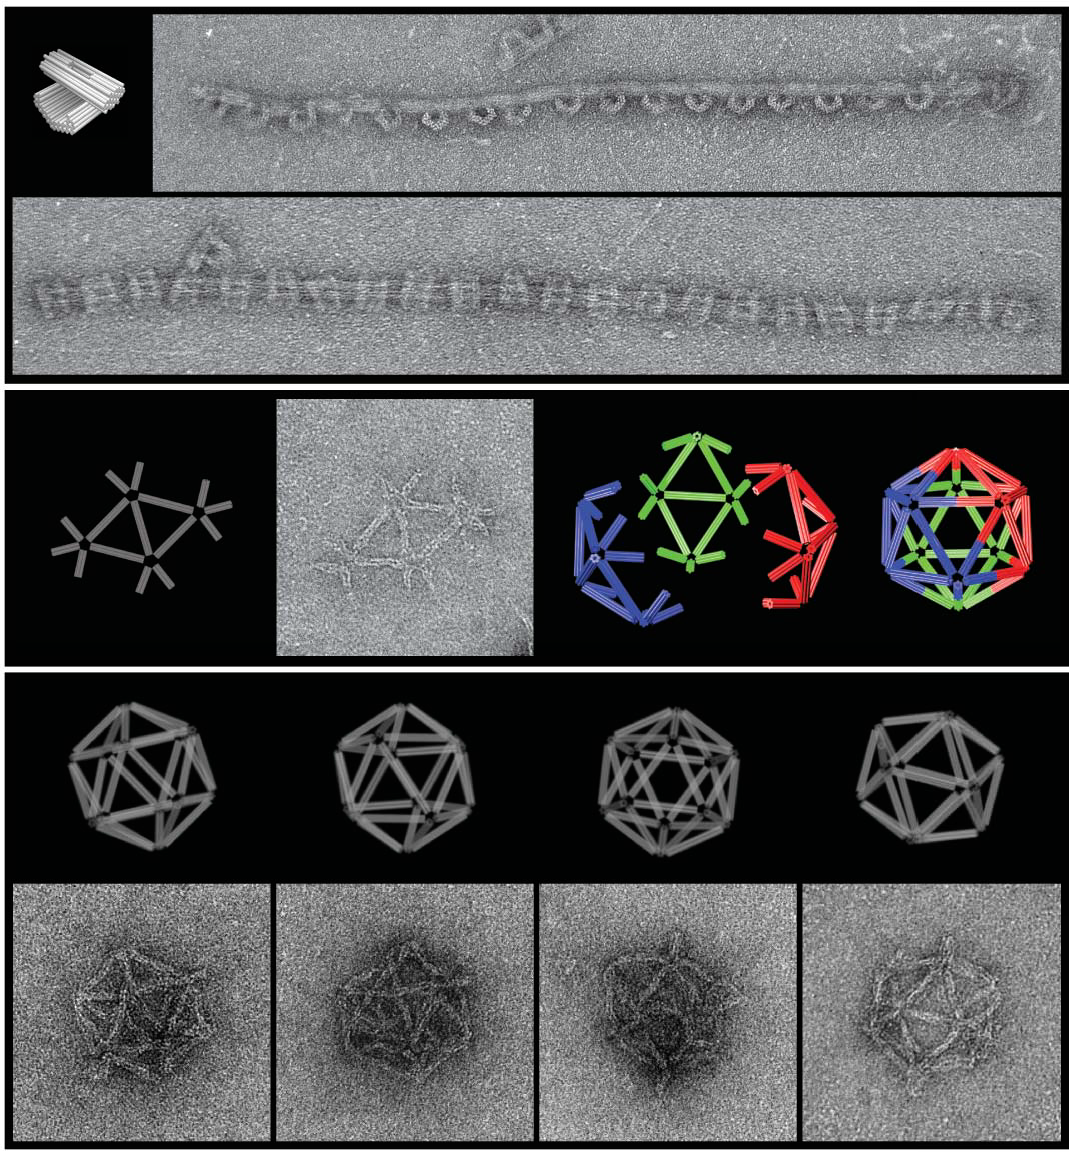
\includegraphics[width=\linewidth]{figures/3D_DNA_origami.png}
			\caption{3D DNA origami from a follow-up paper, \cite{douglas2009self}}
		\end{subfigure}
	
	\end{figure}
\end{frame}

\begin{frame}{From DNA origami to polypeptide origami}
	\begin{itemize}
		\item Advantages of using polypeptides over DNA
		\begin{itemize}
			\item Custom DNA synthesis becomes expensive very quickly
			\item More diversity in the available number of functional groups (20 amino acids vs 4 nucleotides) \cite{kovcar2015topofold}
			\item Possibility of in-vivo production and folding 
		\end{itemize}
		\item We need a class of peptides that is both flexible and understood well-enough, so that we can predict whether and how will they bind
	\end{itemize}
\end{frame}

\begin{frame}{Coiled coils}
	\begin{columns}[T] % align columns
		\begin{column}{.48\textwidth}
				\begin{itemize}
				\item Building blocks are heptads (7 amino acids), positions within heptad denoted with \emph{abcdefg}
				\item Empirical models developed for estimating the interaction free energy (``interaction score''), based solely on primary structure \cite{fong2004predicting, potapov2015data}
				\[ \mathrm{score} = \mathrm{weights} \cdot \mathrm{features} \]
			\end{itemize}
		\end{column}%
		\hfill%
		\begin{column}{.48\textwidth}
			\begin{figure}
				\centering
				\hspace{-1.05cm}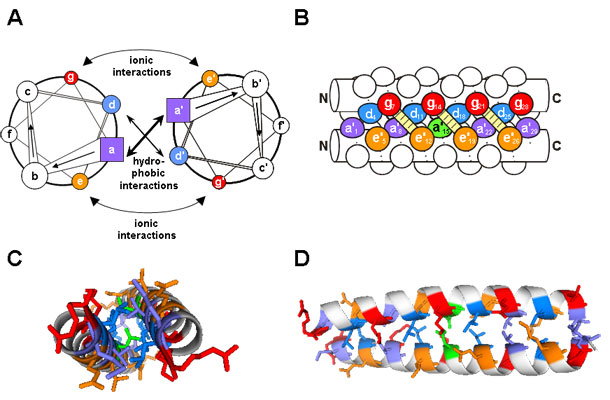
\includegraphics[width=1.2\linewidth]{figures/bCIPA_cc_complete}
				\caption{Different views of coiled-coil dimers}
			\end{figure}
		\end{column}%
	\end{columns}
	
\end{frame}

\begin{frame}{Single-chain polypeptide tetrahedron \cite{gradivsar2013design}}
	%Story: the first paper that actually managed to construct something useful with Coiled-Coils is this one. They designed a long chain, which has naturally folded into a tetrahedron...
	\begin{figure}
		\centering
		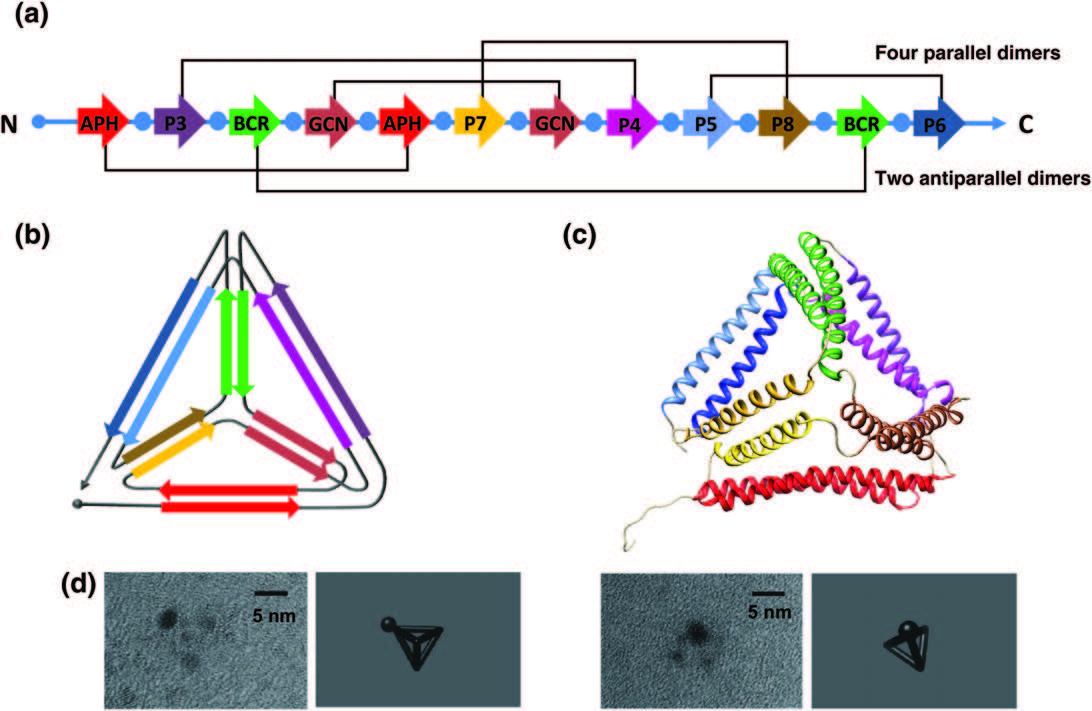
\includegraphics[width=\linewidth]{figures/tetrahedron_process}	
		\caption{Construction steps for the tetrahedron}
		\label{fig:tetrahedron}
	\end{figure}
\end{frame}

\begin{frame}{Workflow}
%Draw the graphs on the board
%Prepare a paper with the double trace, so that I can draw it with a red pen on the board
\begin{enumerate}
	\item Design the polyhedron
	\item {\color<3->{blue}Find a suitable double trace of the polyhedron graph} %we know it exists, because the D(G) is Eulerian
	\item \alert<2->{Choose a set of peptides to be placed along the edges} %so that they interact only mutually
	\item Synthesize the peptide chain
	\item Validate the design experimentally
\end{enumerate}
\end{frame}

\section{Orthogonal sets}

\begin{frame}{Preliminaries}
	\begin{itemize}
		\item Let $G$ be a polyhedron graph with $n$ vertices and $m$ edges, that we want to realize as a single chain -- we need $m$ pairs of peptides that interact only mutually
		\item We search for these pairs inside a (large) set of admissible peptides, $A$. The interactions between them are represented as a matrix $M$ -- the \emph{interaction matrix}.
		\item Given $c_s, c_w \in \mathbb R$, construct the \emph{interaction graph} $G_i = (V, E, E_s)$
		\begin{enumerate}[i)]
			\item $V = A$ (the set of peptides);
			\item $E = \{ \{i, j\} | M_{ij} \leq c_w \}$ (the set of all interacting peptide-pairs) 
			\item $E_s = \{ \{i, j\} | M_{ij} \leq c_s \}$ (the set of all strongly interacting peptide-pairs/edges)
		\end{enumerate}
	\end{itemize}
\end{frame}

\begin{frame}{Interaction graphs}
\begin{figure}[h]
	\centering
	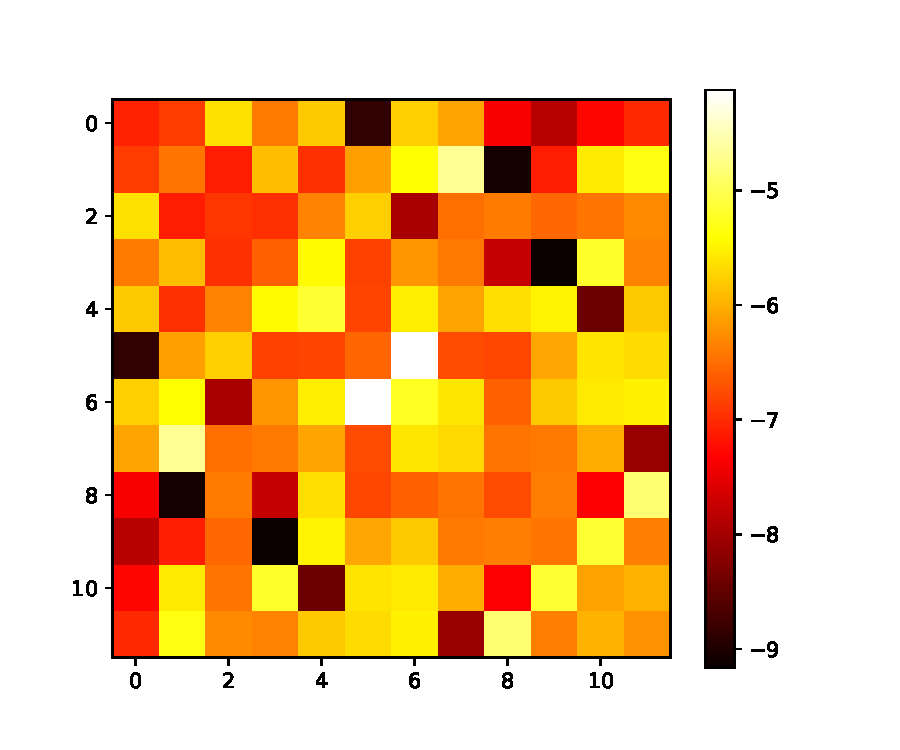
\includegraphics[width=0.7\linewidth]{interaction_matrix_full.pdf}
	\caption{Full interaction matrix}
\end{figure}
\end{frame}

\begin{frame}{Interaction graphs}
\begin{figure}[h]
	\centering
	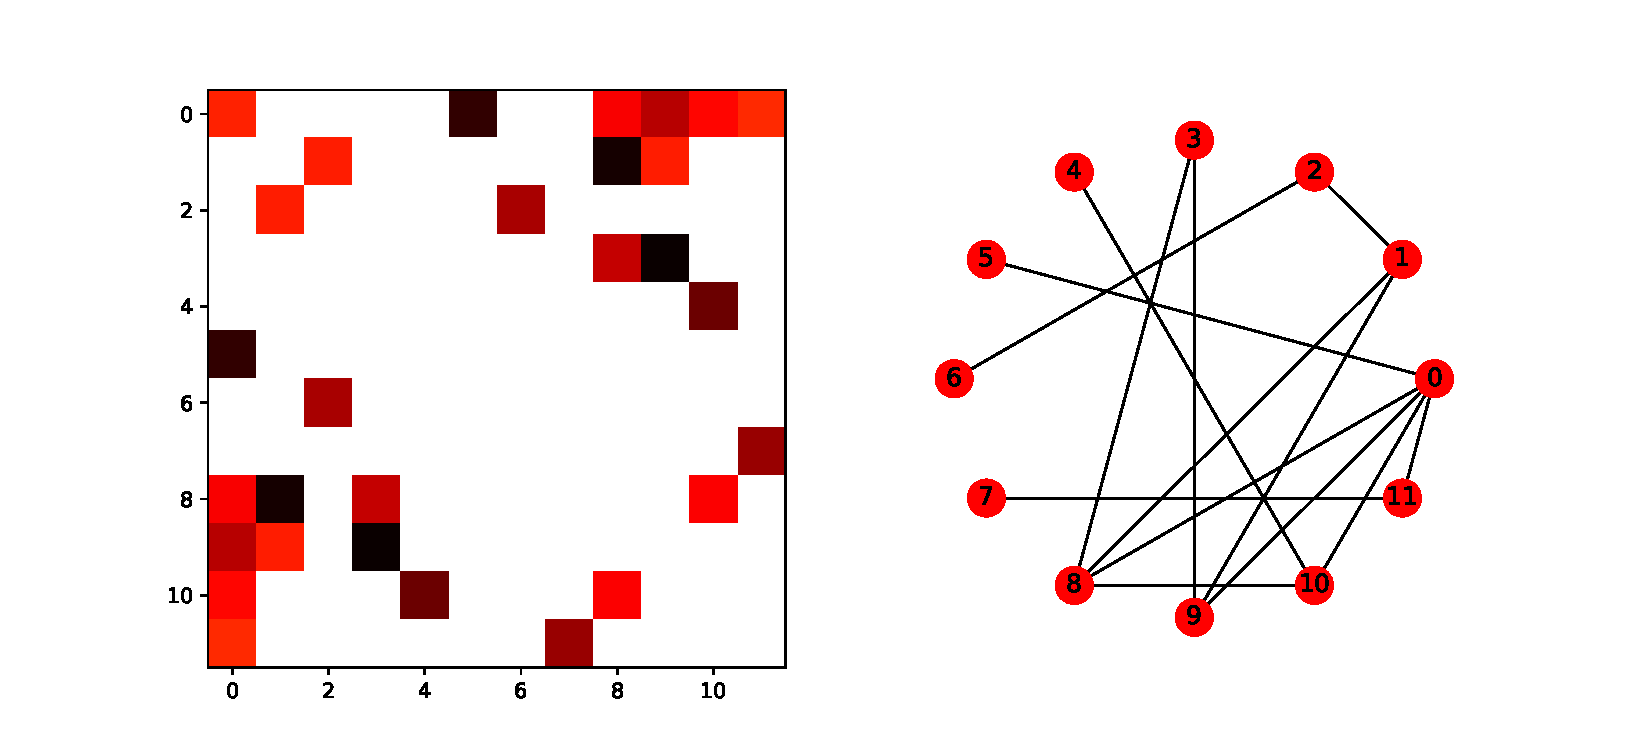
\includegraphics[width=\linewidth]{interaction_matrix_edges.pdf}
	\caption{Edges of the interaction graph}
\end{figure}
\end{frame}

\begin{frame}{Interaction graphs}
\begin{figure}[h]
	\centering
	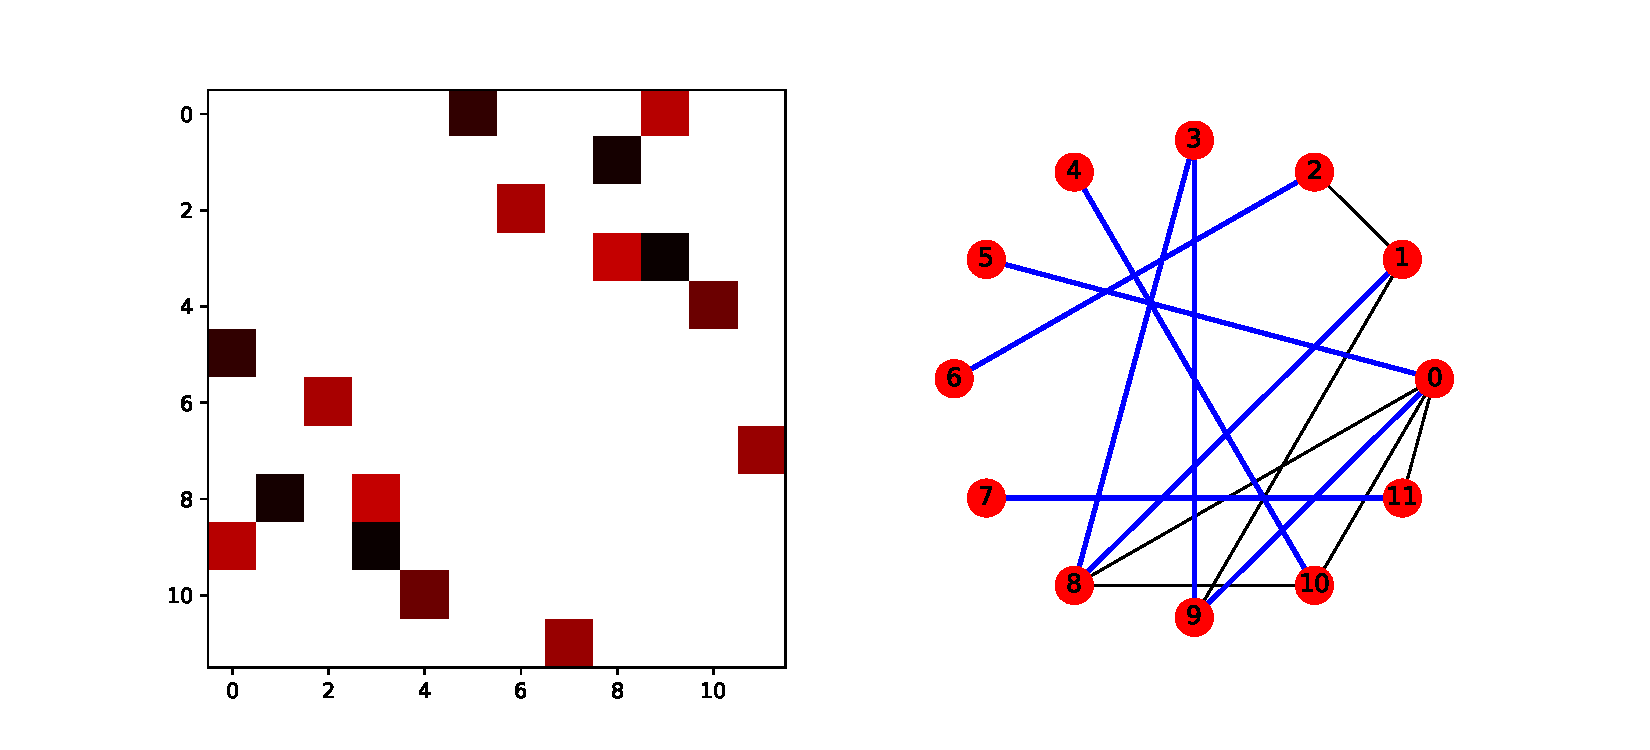
\includegraphics[width=\linewidth]{interaction_matrix_strong_edges.pdf}
	\caption{Strong edges of the interaction graph}
\end{figure}
\end{frame}

\begin{frame}{Interaction graphs}
\begin{figure}[h]
	\centering
	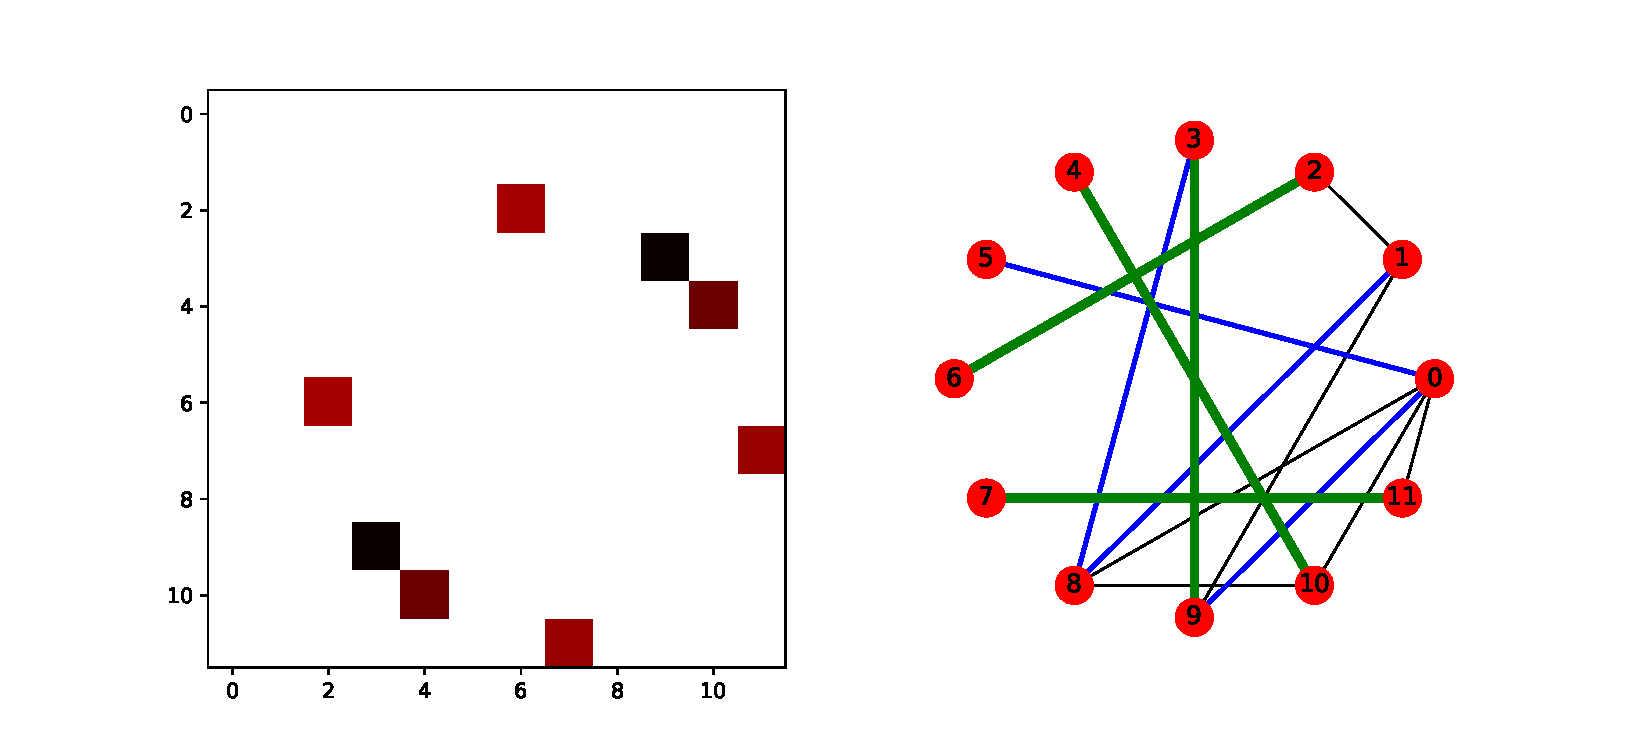
\includegraphics[width=\linewidth]{interaction_matrix_independent_edges.pdf}
	\caption{Independent edges of the interaction graph}
\end{figure}
\end{frame}

\begin{frame}{Definition}
	We can define such a set of edges for any graph $G=(V, E)$ and a set $E_s \subseteq E$
	\begin{block}{Orthogonal set definition}
		A subset $S \subseteq E_s$ is an \emph{orthogonal set} if for any two distinct edges $u_1v_1, u_2v_2 \in S$ the following holds:
		\begin{enumerate}[i)]
			\item The two edges are not incident to each other, i.e. $\{u_1,v_1\} \cap \{u_2, v_2\} = \emptyset.$
			\item The two edges are not incident to a common edge, that is, \[\{u_1u_2,\; u_1v_2,\; v_1u_2,\; v_1v_2\} \cap E = \emptyset.\]
			\item Additionally, if $u_1 \neq v_1$ (i.e. the edge is not a loop), we require that $u_1$ and $v_1$ are not incident to any loops in $E$. 
		\end{enumerate}
	\end{block}
\end{frame}

\begin{frame}{Orthogonal sets -- original results \cite{brodnik2016construction}}
	Similarly to the maximum independent set (MIS) problem, we define the maximum orthogonal set (MOS) problem to be the tuple $(V, E, E_s, k)$, and prove the following
	\begin{theorem}
		The Maximum Orthogonal Set Problem is NP-complete.
	\end{theorem}
	\begin{proof}[Proof idea]
		Starting from $G=(V, E)$, form $G'=(V', E')$ by adding $v'$ for every $v \in V$, and connecting it only to the corresponding $v$. Prove that the MOS in $G'$ consists only of edges of the form $vv'$. Then the $v$-endpoints of these edges form a MIS in $G$. Also, a MIS in $G$ gives a MOS in $G'$.
	\end{proof}
\end{frame}

\begin{frame}{Exact algorithm for orthogonal sets}
\begin{enumerate}
	\item Start with a graph $G = (V, E)$ and a set $E_s \subseteq E$ (e.g. an interaction graph)
	\item From $E_s$ remove all pairs $uv$ where $u \neq v$ and $u$ or $v$ is incident to a loop
	\item Form a new graph $G' = (E_s, E')$, where we connect two vertices $u_1v_1$ and $u_2v_2$ if they can not be together in an orthogonal set
	\item Find the maximum independent set in $G'$ (= the maximum orthogonal set in $G$)
\end{enumerate}
\end{frame}

\begin{frame}{Some orthogonal sets}
	11-, and 21-pair orthogonal sets were constructed, currently undergoing experimental validation.
	\begin{figure}
		\centering
		\begin{subfigure}{0.45\textwidth}
			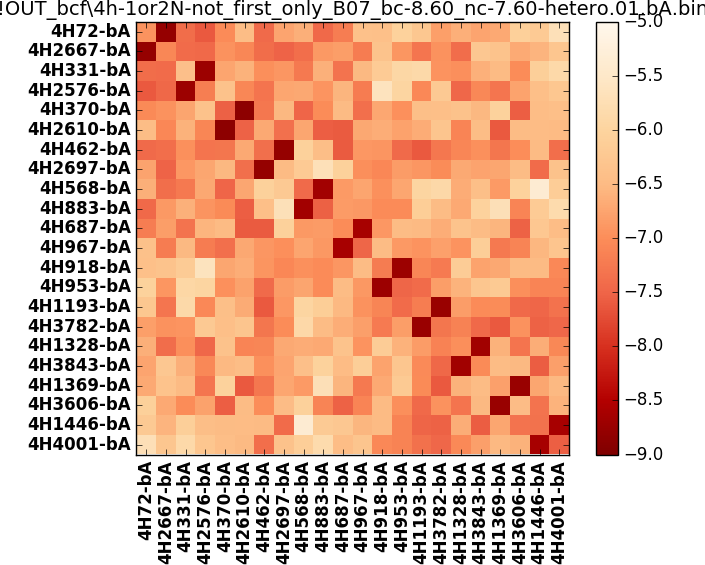
\includegraphics[width=\linewidth]{figures/hetero_scores}
			\caption{Heterodimers only}
		\end{subfigure}
		~
		\begin{subfigure}{0.45\textwidth}
			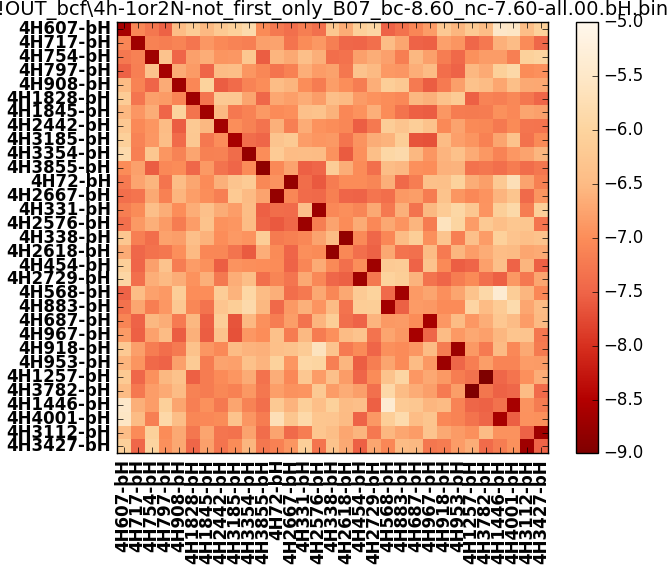
\includegraphics[width=\linewidth]{figures/hetero_+_homo_scores}
			\caption{Both homodimers and heterodimers}
		\end{subfigure}
	\caption{Interaction scores for the constructed orthogonal sets}
	\end{figure}
\end{frame}

\section{Heuristics}
\begin{frame}{The need for heuristics}
	\begin{itemize}
		\item Clique computation is still computationally expensive
		\item Instead of considering a large initial set of peptides, and finding the largest orthogonal subset, try to build the orthogonal set directly
		\item Two greedy approaches
		\begin{enumerate}
			\item Start from a small library of heptads. Greedily build longer peptide pairs, by adding pairs of heptads that are known to bind to each-other.
			\item \alert<2>{Iteratively extend a small orthogonal set, by alternatively taking its Cartesian
			product with another set, and determining the maximum orthogonal subset of the
			(still moderately sized) resulting product set.}
		\end{enumerate}
	\end{itemize}
\end{frame}

\begin{frame}{Iterative set building}
\begin{itemize}
	\item The algorithm fits into the intensification-diversification framework for combinatorial optimization metaheuristics
	\begin{description}
		\item[diversification:] Explore the search space, by taking the ``Cartesian product''
		\[ S_k \cdot H_{k+1} = \{ a\cdot b | a \in S_k, b \in H_{k+1} \} \]
		\item[intensification:] Exploit the accumulated knowledge about the search space
		\[ S_{k+1} = \mathrm{OrthogonalSubset}(S_k \cdot H_{k+1}) \]
	\end{description}
	\item $S_k$ and $H_k$ are the current orthogonal set, and the current \emph{extension set}, respectively 
\end{itemize}
\end{frame}

\begin{frame}{One more orthogonal set}
\begin{figure}[h]
	\centering
	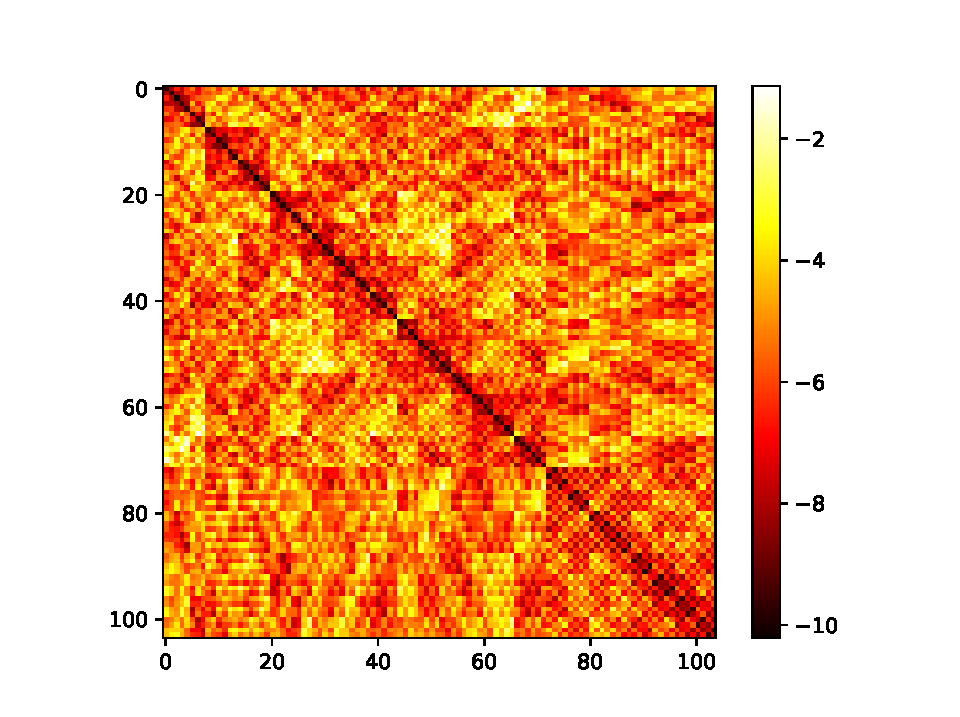
\includegraphics[width=0.8\linewidth]{interaction_matrix_hexaheptad.pdf}
	\caption{A 104-peptide orthogonal set, obtained using the previously described algorithm}
\end{figure}
\end{frame}

\section{Results and conclusions}

\begin{frame}{Results and conclusions}
	\begin{itemize}
		\item Significance of molecular self-assembly techniques
		\item Methods for doing polypeptide origami with coiled coils
		\item Algorithmic way of determining an orthogonal subset
		\item Heuristics for building orthogonal sets directly 
		\item Possible applications to independent sets of product graphs?
	\end{itemize}
\end{frame}

\begin{frame}[plain,c]
	\begin{center}
		\Huge Questions?
	\end{center}
\end{frame}

\begin{frame}[plain,c]
	\begin{center}
		\Huge Thank you for your attention!
	\end{center}
\end{frame}

\begin{frame}[allowframebreaks]{Bibliography}
	\bibliographystyle{plain}
	\bibliography{../thesis/bibliography}
\end{frame}

\end{document}